% !TeX program = pdflatex
\documentclass[border=6pt]{standalone}
\usepackage{tikz}
\usetikzlibrary{arrows.meta, positioning}
\usepackage{amssymb}
\definecolor{MediumRed}{rgb}{0.925, 0.345, 0.345}
\definecolor{MediumGreen}{rgb}{0.37, 0.7, 0.66}
\definecolor{MediumBlue}{rgb}{0.015, 0.315, 0.45}
\definecolor{DarkBlue}{rgb}{0.05, 0.15, 0.35}

\begin{document}
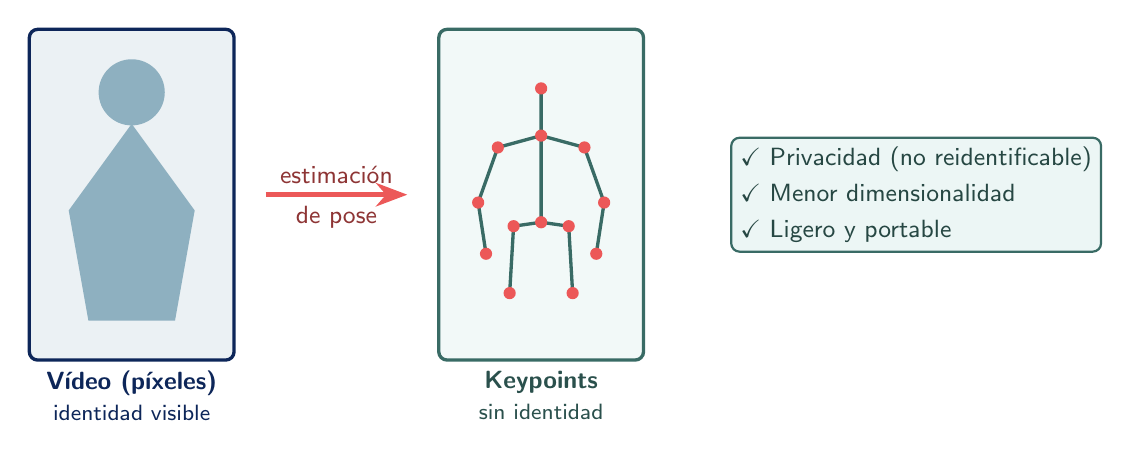
\begin{tikzpicture}[font=\sffamily]

% ================= IZQUIERDA: vídeo (píxeles) =================
\begin{scope}[shift={(0,0)}]
    \fill[MediumBlue!8, draw=DarkBlue, very thick, rounded corners=3pt]
        (-1.3,-2.1) rectangle (1.3,2.1);
    % silueta (identidad visible)
    \fill[MediumBlue!45] (0,1.3) circle (0.42);                 % cabeza
    \fill[MediumBlue!45] (0,0.9) -- (0.8,-0.2) -- (0.55,-1.6)
        -- (-0.55,-1.6) -- (-0.8,-0.2) -- cycle;               % cuerpo
    \node[align=center, font=\sffamily\small, text=DarkBlue] at (0,-2.55)
        {\textbf{Vídeo (píxeles)}\\\footnotesize identidad visible};
\end{scope}

% ================= FLECHA: estimación de pose =================
\draw[-{Stealth[length=4mm]}, line width=1.6pt, MediumRed]
    (1.7,0) -- node[above, font=\sffamily\small, text=MediumRed!60!black]
    {estimación} node[below, font=\sffamily\small, text=MediumRed!60!black]
    {de pose} (3.5,0);

% ================= DERECHA: keypoints (esqueleto) =================
\begin{scope}[shift={(5.2,0)}]
    \fill[MediumGreen!8, draw=MediumGreen!60!black, very thick, rounded corners=3pt]
        (-1.3,-2.1) rectangle (1.3,2.1);
    % coordenadas del esqueleto
    \coordinate (head)  at (0,1.35);
    \coordinate (neck)  at (0,0.75);
    \coordinate (lsh)   at (-0.55,0.6);
    \coordinate (rsh)   at (0.55,0.6);
    \coordinate (lel)   at (-0.8,-0.1);
    \coordinate (rel)   at (0.8,-0.1);
    \coordinate (lha)   at (-0.7,-0.75);
    \coordinate (rha)   at (0.7,-0.75);
    \coordinate (hip)   at (0,-0.35);
    \coordinate (lhi)   at (-0.35,-0.4);
    \coordinate (rhi)   at (0.35,-0.4);
    \coordinate (lkn)   at (-0.4,-1.25);
    \coordinate (rkn)   at (0.4,-1.25);
    % huesos
    \draw[MediumGreen!60!black, line width=1.2pt]
        (head)--(neck) (neck)--(lsh) (neck)--(rsh)
        (lsh)--(lel)--(lha) (rsh)--(rel)--(rha)
        (neck)--(hip) (hip)--(lhi)--(lkn) (hip)--(rhi)--(rkn);
    % keypoints
    \foreach \p in {head,neck,lsh,rsh,lel,rel,lha,rha,hip,lhi,rhi,lkn,rkn}
        \fill[MediumRed] (\p) circle (2.2pt);
    \node[align=center, font=\sffamily\small, text=MediumGreen!45!black] at (0,-2.55)
        {\textbf{Keypoints}\\\footnotesize sin identidad};
\end{scope}

% ================= VENTAJAS =================
\node[draw=MediumGreen!60!black, thick, rounded corners=3pt, fill=MediumGreen!12,
      align=left, text=MediumGreen!40!black, font=\sffamily\small,
      right=1.1cm of {(6.5,0)}] (adv)
    {$\checkmark$ Privacidad (no reidentificable)\\[2pt]
     $\checkmark$ Menor dimensionalidad\\[2pt]
     $\checkmark$ Ligero y portable};

\end{tikzpicture}
\end{document}
